\section{Definition}
\subsection{Datenbankmodell}
\subsubsection{Entity Relationship Modell (ERM)}
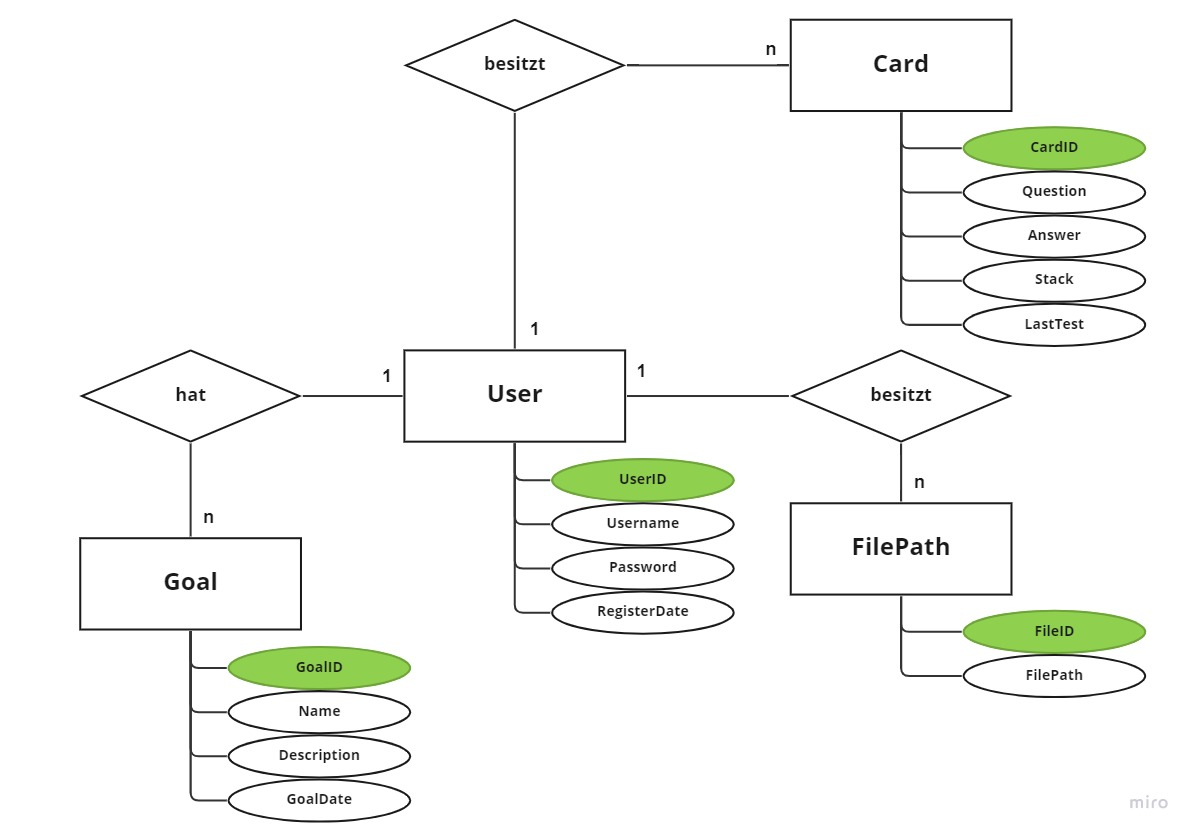
\includegraphics[width=1\textwidth]{images/ERM.jpg}
\newpage

\subsubsection{Data Dictionary}
\begin{table}[]
    \centering
    \resizebox{\columnwidth}{!}{%
    \begin{tabular}{|c|c|c|l|c|c|l|}
    \hline
    \textbf{Attribut} & \textbf{Datentyp} & \textbf{Länge} & \textbf{Null} & \textbf{Default} & \textbf{Schlüssel} & \textbf{Beschreibung} \\ \hline
    UserID       & INTEGER & -  & \multicolumn{1}{c|}{Nein} & - & P & ID des Benutzers                  \\ \hline
    Username     & VARCHAR & 40 & Nein                      & - & - & Name des Benutzers                \\ \hline
    Password     & VARCHAR & 30 & Nein                      & - & - & Passwort des Benutzers            \\ \hline
    RegisterDate & DATE    & -  & Nein                      & - & - & Registrierungsdatum des Benutzers \\ \hline
    \end{tabular}%
    }
\end{table}

% Please add the following required packages to your document preamble:
% \usepackage{graphicx}
\begin{table}[]
    \centering
    \resizebox{\columnwidth}{!}{%
    \begin{tabular}{|c|c|c|l|c|c|l|}
    \hline
    \textbf{Attribut} &
      \textbf{Datentyp} &
      \textbf{Länge} &
      \textbf{Null} &
      \textbf{Default} &
      \textbf{Schlüssel} &
      \textbf{Beschreibung} \\ \hline
    GoalID      & INTEGER & - & \multicolumn{1}{c|}{Nein} & - & P & ID des Lernziels           \\ \hline
    Name        & VARCHAR & - & Nein                      & - & - & Name des Lernziels         \\ \hline
    Description & VARCHAR & - & Nein                      & - & - & Beschreibung des Lernziels \\ \hline
    GoalDate &
      DATE &
      - &
      Nein &
      - &
      - &
      \begin{tabular}[c]{@{}l@{}}Datum bis wann das Lernziel erreicht \\  werden soll\end{tabular} \\ \hline
    \end{tabular}%
    }
\end{table}

% Please add the following required packages to your document preamble:
% \usepackage{graphicx}
\begin{table}[]
    \centering
    \resizebox{\columnwidth}{!}{%
    \begin{tabular}{|c|c|c|c|c|c|l|}
    \hline
    \textbf{Attribut} &
      \textbf{Datentyp} &
      \textbf{Länge} &
      \textbf{Null} &
      \textbf{Default} &
      \textbf{Schlüssel} &
      \textbf{Beschreibung} \\ \hline
    CardID &
      INTEGER &
      - &
      Nein &
      - &
      P &
      ID einer Lern-Karteikarte \\ \hline
    Question &
      VARCHAR &
      - &
      Nein &
      - &
      - &
      Frage einer Lern-Karteikarte \\ \hline
    Answer &
      VARCHAR &
      - &
      Nein &
      - &
      - &
      Antwort einer Lern-Karteikarte \\ \hline
    Stack &
      INTEGER &
      - &
      Nein &
      1 &
      - &
      \begin{tabular}[c]{@{}l@{}}Gibt an in welchen Stapel sich\\ die Lern-Karteikarte befindet\end{tabular} \\ \hline
    \multicolumn{1}{|l|}{LastTest} &
      \multicolumn{1}{l|}{BOOLEAN} &
      \multicolumn{1}{l|}{-} &
      Ja &
      - &
      - &
      \begin{tabular}[c]{@{}l@{}}Gibt an, ob die Lern-Karteikarte\\ bei der letzten Prüfung erfolgreich\\ beantwortet wurde\end{tabular} \\ \hline
    \end{tabular}%
    }
\end{table}

\begin{table}[]
    \centering
    \resizebox{\columnwidth}{!}{%
    \begin{tabular}{|c|c|c|c|c|c|l|}
    \hline
    \textbf{Attribut} &
      \textbf{Datentyp} &
      \textbf{Länge} &
      \textbf{Null} &
      \textbf{Default} &
      \textbf{Schlüssel} &
      \textbf{Beschreibung} \\ \hline
    FileID &
      INTEGER &
      - &
      Nein &
      - &
      P &
      ID eines Datei-Pfades \\ \hline
    FilePath &
      VARCHAR &
      - &
      Nein &
      - &
      - &
      \begin{tabular}[c]{@{}l@{}}Der zugehörige Pfad einer Datei.\\ Dateien können Skripte sein.\end{tabular} \\ \hline
    \end{tabular}%
    }
\end{table}
